
%%%%%%%%%%%%%%%%%%%%%%% file typeinst.tex %%%%%%%%%%%%%%%%%%%%%%%%%
%
% This is the LaTeX source for the instructions to authors using
% the LaTeX document class 'llncs.cls' for contributions to
% the Lecture Notes in Computer Sciences series.
% http://www.springer.com/lncs       Springer Heidelberg 2006/05/04
%
% It may be used as a template for your own input - copy it
% to a new file with a new name and use it as the basis
% for your article.
%
% NB: the document class 'llncs' has its own and detailed documentation, see
% ftp://ftp.springer.de/data/pubftp/pub/tex/latex/llncs/latex2e/llncsdoc.pdf
%
%%%%%%%%%%%%%%%%%%%%%%%%%%%%%%%%%%%%%%%%%%%%%%%%%%%%%%%%%%%%%%%%%%%


\documentclass[runningheads,a4paper]{llncs}

\usepackage{amssymb}
\setcounter{tocdepth}{3}
\usepackage{graphicx}
\usepackage{url}
\urldef{\mailsa}\path|{alfred.hofmann, ursula.barth, ingrid.haas, frank.holzwarth,|
\urldef{\mailsb}\path|anna.kramer, leonie.kunz, christine.reiss, nicole.sator,|
\urldef{\mailsc}\path|erika.siebert-cole, peter.strasser, lncs}@springer.com|    
\newcommand{\keywords}[1]{\par\addvspace\baselineskip
\noindent\keywordname\enspace\ignorespaces#1}


\usepackage{listings}
\usepackage{xcolor}
\usepackage{textcomp}
\usepackage{geometry}
\usepackage{pdflscape}

\usepackage{selinput}
\SelectInputMappings{   % Semi-automatic determination
               % of input encoding
  oslash={ø},           % by a list of selected glyphs
	              % see: http://partners.adobe.com/public/developer/en/opentype/glyphlist.txt
}


\begin{document}

\mainmatter  % start of an individual contribution

% first the title is needed
\title{Project in Personal Data Interaction:\\FriendBump}

% a short form should be given in case it is too long for the running head
\titlerunning{Project in Personal Data Interaction: FriendBump}

% the name(s) of the author(s) follow(s) next
%
% NB: Chinese authors should write their first names(s) in front of
% their surnames. This ensures that the names appear correctly in
% the running heads and the author index.
%
\author{S\o ren Howe Gersager \and Anders L\o nberg Rahbek}
%
\authorrunning{Project in Personal Data Interaction: FriendBump}
% (feature abused for this document to repeat the title also on left hand pages)

% the affiliations are given next; don't give your e-mail address
% unless you accept that it will be published
\institute{DTU Compute, Technical University of Denmark, \\Richard Petersens Plads, Building 324, 2800 Kgs. Lyngby, Denmark \\
%\mailsa\\
%\mailsb\\
%\mailsc\\
\url{http://www.compute.dtu.dk/}}

%
% NB: a more complex sample for affiliations and the mapping to the
% corresponding authors can be found in the file "llncs.dem"
% (search for the string "\mainmatter" where a contribution starts).
% "llncs.dem" accompanies the document class "llncs.cls".
%

\toctitle{Lecture Notes in Computer Science}
\tocauthor{Authors' Instructions}
\maketitle


\begin{abstract}
The abstract should summarize the contents of the paper and should
contain at least 70 and at most 150 words. It should be written using the
\emph{abstract} environment.
\keywords{geolocation·android·prototyping·app·evaluation}
\end{abstract}


\section*{Preface}
This report is produced based on a course project in Personal Data Interaction on the Technical University of Denmark. The references are stated with a number in brackets eg. [1]. If the reference is placed after the period in a section, the reference is used as reference for the entire section. 
Both authors are responsible for the entire content of this report.


\section{Introduction}
Many of us has tried to go shopping, been to a conference or a concert, where you came home and discovered that one of your friends had also been there. If you had known that he would be there, you could’ve met with him and possibly made the experience more enjoyable.\\

This leaves us with the following problem definition: You don’t know when a friend is nearby but you would like to know in certain situations. \\

This problem can be solved by a personal app, that allows you to  broadcasts your location to your friends and your friends location to you, which enables you to quickly contact them when you are close to each other.\\

In this report we will describe the process of developing a prototype solution to solve this problem.
We start with related works to describe how our app differs from other similar solutions in the market. 
We analyse our problem further and then describe our design for the app. We evaluate the design, after describing the implementation. \\
Finally we go through our results and discuss them. Last, some remarks for possible future work on the app and a conclusion. 

\section{Analysis}
As the problem is, that you don’t know if a friend is nearby, the immediate solution would be to continuously broadcast your location to your friends.
However we have to factor in privacy and avoid giving the users the feeling of being spied on. People will probably not use a solution that allows everyone to see their location at all times. The location should only be broadcast if friends are within a certain radius.\\
Also we figured the user should be able to disable broadcasts temporarily, because there are times when you don't want to advise your location, like going to the doctors or on a date where you’d rather be incognito.
The solution would have to work in an outdoors context while on foot, smartwatch support could contribute to this. The watch is more convenient if you're out shopping or performing another activity without your hands being free, as being notified is much easier in that setting.

\section{Design}\label{design}
Our design methods is divided into two overall parts: a lo-fi prototype which is is developed based on an initial user story map (see figure \ref{fig:user_story_mapping}) and done with mock-ups, and a hi-fi prototype, an Android app with Android Wear notifications. The hi-fi prototype is based on the lo-fi prototype. 

\subsection{Lo-fi prototype}
We wanted to create a fixed-path prototype, which allowed for interaction by users early as explained in \cite{prototyping}. We used an online wireframe mockup tool\cite{ninja}, which allowed us to quickly sketch out designs for validation. \\


We wanted the following features for our first prototype: 
\begin{itemize}
  \item A map to see where our friends are 
	\item A list with those friends to give the user a better overview over these friends. 
	\item A text-field which told the user how many friends that’s near him
	\item An icon in the list, to show which network the friend is from
	\item Distance to each of the friends
	\item When (and maybe what) the friend has made an update on the particular social network.
	\item A button to toggle the broadcast on and off\\ 
\end{itemize}

Because our number of features were relatively modest, we tried to minimize the number of touches and taps you'd have to do to get to a wanted feature. These features are sketched in figure \ref{fig:lo-fi-fixed-panel-simple-marker}.

We found out through feedback that calling and texting a friend in-app as well as navigating to him was a wanted feature. Also markers in form of profile image from a social network would help the user to visually find a friend quicker. This can be seen in figure \ref{fig:lo-fi-w.navigation}. 

In the early prototypes the friend list was always visible (non-slide) (figure \ref{fig:lo-fi-fixed-panel}) for accessing it quickly, but after a quick \& dirty evaluation (see evaluation), we changed it to a slide up panel. This was to increase the size of the map for the user, which is very important when the "screen real estate" is limited. This design can be seen in figure \ref{fig:lo-fi-panel-collapsed}.

\subsection{Hi-fi prototype}

As the hi-fi prototype is based on the lo-fi, we implemented the design from the last lo-fi prototype. 

We decided that our hi-fi prototype should be more vertical slice than the lo-fi, and thus focus on the primary feature of showing friends on a map, instead of including non-essential features. 

From a quick \& dirty and talk aloud evaluation, we made the following changes and additions:
\textbf{What we changed:}\begin{itemize}
\item Button to toggle broadcast on and off\\
We found out, that people didn’t understand the first broadcast icon tried to convey (top-left icon on figure \ref{fig:lo-fi-panel-collapsed}), so we found another icon based on suggestions from evaluation. \\

\textbf{What we removed:}
\item Updates from network\\
We removed this to make out prototype more vertical and because it was in general a little out of our scope. It was a nice feature but nothing more. \\

\item Text-field\\
We removed the text-field which told the user how many friend there was near him. The user can manage to count some few friend, and the other case with many friend, we found a possible solution using visualization (See section \ref{future-work}). \\

\item Navigation\\
We decided to remove in-app navigation, the feature which shows a proposed path when touching a marker. The reason for this was simply because it would be too timeconsuming to implement.

\end{itemize}

After further development and quick \& dirty, we changed the button to toggle the broadcast on and off and added a nudge button. \\
See the result on figure \ref{fig:hi-fi app friendlist expanded} and \ref{fig:hi-fi app friendlist collapsed}. 

Part of our hi-fi prototype was also Android Wear support, we added notifications and options to SMS and call a friend as seen on figure \ref{fig:hi-fi watch notification collapsed}, \ref{fig:hi-fi watch notification expanded}, \ref{fig:hi-fi watch sms} and \ref{fig:hi-fi watch call}

\section{Implementation}
Our implementation is divided into two parts: the already mentioned app and a backend server. The backend is composed of a python webserver and a RabbitMQ server\cite{rabbitmq}. \\
We will in the following section describe these two parts and details regarding them. 

\subsection{Android app}
Our activity has several functions, which are for communicating with the backend message-queue and common Android functionality. See the sourcecode starting from page \pageref{source-code}. \\
There are a couple of non-trivial functions, which we will describe in a bit more detail below.\\

\underline{drawMarkerBitmap}\\
This function creates a bitmap object containing the initials of the person on a round and red background, for example Anders Rahbek turns into AR.\\

This is used to show an unique marker for a friend, thus the function is been called from “updateMarker” function. \\
The function drawing the bitmap to the marker is based on this code snippet from Stack Overflow\cite{bitmapstackoverflow}

\underline{getNumber}\\
The getNumber function, tries to find a telephone number based on a name. It iterate through the mobiles phonebook and return the number if it finds the name, null otherwise. \\

The function is used to create an action to a notification, so the user can call the friend directly from the notification. It is also used to call and sms from the list, under a person. 
The code is strong inspired of the code from \cite{number}.\\


To give a sense on how some of the functions work together, we have made some sequence diagrams, to show the flow. These diagrams is figure \ref{fig:sq-onLocation} and \ref{fig:sq-nudge}.\\ 

For the app we used the following libraries: Paho MQTT\cite{paho}, Sothee Sliding up panel\cite{slidinguppanel}.


\subsection{Backend (RabbitMQ and Flask)}
The Python web server is running a simple Flask\cite{flask} script which can be queried with an email and then returns a list of predetermined friends in JSON format, we decided to use these tools because they allowed us to quickly set up a “mock” backend for the app to communicate with. While testing the app among a number of users, we simply modified the script to return a number of their chosen friends based on their email.\\

The RabbitMQ is responsible for acting as a message queue for relaying the messages between devices running the app. The protocol used for the messages is MQTT, which was chosen because it’s lightweight in terms of code footprint and network bandwidth. The message queue use the notion of “topics”, so each message is broadcast on a topic, which in our case is the email of the user and the latitude and longitude of their location reduced to 2 decimal places. This reduces the number of updates received by the app since you do not receive an update from a friend if your location is not the same as theirs to 2 decimal places. In hindsight this could also be implemented server-side where the server compared the last location with all friends, and only relayed it if they were within radius of each other.

 
\section{Related works}
\textbf{Find My Friends \& Buddies by Sygic - FMFB (updated 2014, Google Play, free)}\\
This is an app for locating your friends in real-time much like our app. What is different is the built-in minimum radius our app has, thus you are not able to see your friends location at all times. Furthermore FMFB allows you to see the movement of your friends for the last week, this is intrusive in our opinion and we do not allow that.\\

\textbf{Family Locator by Life360 (updated 2015, Google Play, Free)}\\
Family Locator is similar to our app in the sense that it allows you to see the location of other people, the way ours differ is that their solution are marketed to families or more precisely parents who want to get updated on their children's location, and thus they are also able to see their positions at all times. 


\section{Evaluation}
\subsection*{Quick \& dirty}
As quick \& dirty typically is a formative evaluation method, we used it to get feedback from our fellow students early in the design phase - see section \ref{design} for the result.

\subsection*{Think aloud}
We did two Think aloud evaluations: One formative and one summative.

In both of the them, we used the same tasks to the user. These were the following: 

\begin{itemize}
\item Can the user track and find a friend? 
\item Can the user turn on/off location broadcasts? 
\item Can the user track a friend from a notification?
\item Can the user SMS/call/nudge a friend from the app?
\item Can the user call a friend from a notification?
\item Can the user asses the distance from a given user?
\end{itemize}
The result of the Think aloud evaluation can be found section \ref{result}. 

Both in the formative and summative, we wanted to assess the usability of our design. In the formative, we used our lo-fi, while the summative session was conducted on our hi-fi prototype in an outdoors context to simulate a natural situation our app might be used in.\\
We conducted the summative with an indirect observation technique, where we recorded what the user said. See the transcript of the record on page \pageref{transcript}. \\
The formative was simply conducted with the observer writes the result down. 


\subsection*{Heuristic}
We did a heuristic evaluation on the hi-fi prototype. A fully description of the evaluation and its result, can be found on page \pageref{heuristic}. \\
An summary of the result can be found in section \ref{result}.
\section{Result}\label{result}
\subsection*{Think aloud}

\subsubsection*{Formative}
From this evaluation, we identified the following usability problems:
\begin{itemize}
\item \textbf{Can the user turn on/off location broadcasts?}\\
	The user simply couldn't understand the icon. This is a clear indication, that we need another icon for conveying broadcasting. \\
\item \textbf{Can the user nudge a friend from the app?}\\
The user was in doubt of the icon. He thought it looked very similar to the Facebook nudge icon, so he thought it was a nudge on Facebook - not in the app. This was an indication of we had to change the icon, so it's different from Facebooks. 
\end{itemize}

\subsubsection*{Summative}

From the recorded evaluation (see transcript on page \pageref{transcript}), we identified the following usability problems:

\begin{itemize}
\item \textbf{Can the user turn on/off location broadcasts?}\\
	The user thought the button icon for the button toggling the broadcast, was an icon for sound (probably a speaker icon). This is a clear indication, that we need another icon for conveying broadcasting. \\
	Our user suggested that we could use the same icon as the Facebook Messenger app uses, to turn geolocation on and off, we think it's a reasonable idea. 
\item \textbf{Can the user call a friend from a notification?}\\
	The user had some problems with this. He couldn't expand the notification so the call-action button became visible. 
As the notion of expanding a notification is specific for Android, and our user is an iPhone user, we suspect this could be the reason for his confusion, but we can't know for sure.
\end{itemize}

\subsection*{Heuristic}
We did a summative heuristic evaluation (see page \pageref{heuristic}) and the following is short summary of the findings: \\

We found the app met some of the criteria of the heuristics. Although we found our app lacking in the following sections:
\begin{itemize}
\item Better feedback with toasts and a visual indicator for connectivity
\item Other icons for certain buttons (already mentioned in Think aloud evaluation)
\item Compliance with design guidelines for the Android platform
\item Accelerators on the markers for quickly showing options for a given friend.
\item Help to recover from error is needed and help with the use of the app in general.
\end{itemize}
\section{Discussion}
We would like to have used at least five evaluators for the heuristic evaluation as a larger number of evaluators finds more usability problems as J. Nielsen and R. Molic (1990) found.\cite{heuristics}\\
Due to our "improvised" backend, for calling and texting a friend, the app makes the assumption that the friend is located in the phone book with the same name it receives from the backend.\\

As mentioned in the backend section we cannot set the radius ourselves right now as it's based decimal representations on the latitude and longitudes of the users, this limitation can be corrected comparing the last known location of the sender in the backend and only relay the message if it's within a predefined range we can set.\\
Notifications right now happen every time a friend is within radius and the app is in the background, this is of course not ideal for situations where a sudden influx of friends happen. Notifications could also annoy the user when a friend is constantly going in and out of their radius. We realize notifications are hard to get right but propose the following restrictions on notifications: Only one notification per person per day, If a number of users are in a new area, the notifications will be batched into one, listing all of their names.
\section{Future work}\label{future-work}
From the feedback we received future work can be spent on taking the solution in several interesting directions.\\
The solution could filter based on interests rather than friends, so an example could be if you're into skating or playing soccer, you can be notified when people who identify themselves as either type are present at the local soccerfield or skatepark.\\
By integrating with social networks the solution could rank friends by communication and visualize that rank by a different color on the markers as right now only a single color is used.\\
We also need a solution when there is many friends in one place - se figure \ref{fig:before-visualization}. Our solution as a lo-fi is, to group friends that are clustered. This could be done with K-means algorithm. Then, visualize these clusters as ovals in different sizes and colors, with the number of friends written on it - see figure \ref{fig:after-visualization}.\\

\section{Conclusions}
We iteratively developed a solution for solving the problem of not being aware of when a friend is nearby. We developed a user story mapping and made a lo-fi prototype based on it. After several iterations of lo-fi prototyping we developed a hi-fi prototype as a proof of concept. We continuously validated the prototypes with feedback from quick \& dirty sessions, think-aloud evaluations and at the end a summative heuristic evaluation using the refined Nielsen heuristics\cite{nielsenheuristics}. From the heuristic evaluation we found a number of usability issues which can be worked on. We have laid the foundation and developed a proof-of-concept app which can be taken in several interesting directions as mentioned in the Future work section.
\begin{thebibliography}{4}

\bibitem{prototyping} M. Beaudouin-Lafon, W. Mackay: Prototyping Tools and Techniques
\bibitem{paho} Paho Project: URL \url{http://eclipse.org/paho/}
\bibitem{slidinguppanel} Android Sliding Up Panel: Github \url{https://github.com/umano/AndroidSlidingUpPanel}
\bibitem{nielsenheuristics}Refined heuristics of J. Nielsen: URL \url{http://www.nngroup.com/articles/ten-usability-heuristics/}
\bibitem{bitmapstackoverflow} Drawing a bitmap on a marker: URL \url{http://stackoverflow.com/questions/18335642/how-to-draw-text-in-default-marker-of-google-map-v2}
\bibitem{ninja} NinjaMock - Mockup tool: URL \url{http://ninjamock.com}
\bibitem{rabbitmq} RabbitMQ - Message Queue Server: URL \url{http://www.rabbitmq.com/}
\bibitem{heuristics}Nielsen, J., and R. Molich. “Heuristic Evaluation of User Interfaces.” SIGCHI Bulletin (1990): 249–256. Print.
\bibitem{number} Search for number in phonebook by name: URL \url{http://stackoverflow.com/questions/18201108/getting-number-and-names-of-contacts-in-android}
\bibitem{flask} Flask microframework: URL \url{http://flask.pocoo.org/}
% bibliography examples:

%\bibitem{proceeding2} Foster, I., Kesselman, C., Nick, J., Tuecke, S.: The Physiology of the
%Grid: an Open Grid Services Architecture for Distributed Systems
%Integration. Technical report, Global Grid Forum (2002)

%\bibitem{url} National Center for Biotechnology Information, \url{http://www.ncbi.nlm.nih.gov}

\end{thebibliography}


\section*{Appendix}

\subsection*{Transcript of summative think aloud evaluation}\label{transcript}
The following \textit{in italic} is the transcript of the recordings of what the evaluator has "thought". The question/task that the observer has given the evaluator, is the following bulletpoints. 

It's worth mentioning that the evaluator were used to use an iPhone and not Android. \\

The evaluator is from now on denoted 'E'. \\
\begin{enumerate}
	\item \textbf{Track friend from notificaton}\\
		{[} Upon the notification arriving{]} \\
		\textit{There is a notification...}\\
		{[}E touch the notification and asked for confirmation on what the task was.{]}\\
		\textit{I can see Søren right next to me}\\
		
	\item \textbf{Call a friend directly from a notification}\\
		{[}Upon the notification arriving{]} \\
		\textit{There is a notification. Søren is near me. Some information appears, can i perhaps long-press the notification? No..}\\
		
		{[}E is stopping and don't know what to do.{]}\\
	
	\item \textbf{SMS a friend from the app}\\
		{[}E has the app open from start{]}\\
		\textit{I pull up the list. Find Søren, press the little SMS-icon}\\
		{[}The default SMS app turns up{]}\\
		\textit{And I'm writing a SMS}\\
		
	\item \textbf{Nudge a friend from the app}\\
		{[}E has the app open from start{]}\\
		\textit{I pull up the friend-list. Ehm... Press on Søren. Then the little finger-icon}\\
		
	\item \textbf{Call a friend from the app}\\
		{[}E has the app open from start{]}\\
		\textit{I have the app in my hand. I pull up the friend-list. Press on Søren and press the phone-icon}\\
		
	\item \textbf{Read the distance to a friend, from the app}\\
		{[}E has the app open from start{]}\\
		\textit{I can see Søren on the map. I pull up the friend-list, I can see that he is approx. 22 meters away.}\\
		
	\item \textbf{Turn broadcast off}\\
		{[}E has the app open from start{]}\\
		\textit{I Explore the app a bit. I pull up the friend-list. Pull it down again. I'm pressing the icon in the upper-right corner, what does it do?, i press the sound-icon... a few times. \\I don't know.}
		
\end{enumerate}

\subsection*{Heuristic evaluation} \label{heuristic}
In the last iteration we have evaluated the app using the Nielsen heuristics\cite{nielsenheuristics}.

We have tested the interface independently using two evaluators, below is a summary of the issues found.\\

\begin{enumerate}
  \item \textbf{Visibility of system status}\\
  Our app keeps the user informed about the status of the app, through visual cues and Android Toast messages, however currently two things can be improved in the app regarding system status:
  \begin{enumerate}
    \item \textbf{Broadcast toggling}\\
    Right now the broadcast icon simply changes when toggling broadcasting, this could be improved further by using a Toast and maybe a more visual approach than the icon changes we use now, like adding a small animation to the icon change when touched, providing a sort of tactile feedback to the user.
    
    \item \textbf{Connectivity problems}\\
    The user can be notified of connectivity problems using Toasts and visual cues. 
We previously used a toast when failing to connect, but it was simply annoying rather than informative if a Toast pop-up every few seconds, telling the user it can’t connect. A timeout could be added, so it can only pop-up once every 5 minutes for example, even better a visual effect could be added so the user is constantly aware of the connectivity of the app, perhaps change the opacity of the screen or make it black and white with a visual indicator that it’s reconnecting.  
  \end{enumerate}
  \item \textbf{Match between system and the real world
}\\
Our app provides the user with system information in a clear, non-domain specific language. For example if the user tries to call the friend from the app and it can’t find the number it simple says \\
"Number not found. Can't make the call!".\\
This also happens with SMS and nudge.
  \item \textbf{User control and freedom}\\
  The sliding up bar can perhaps be activated by mistake, an icon with arrows facing up when slid down and down when slid up, could perhaps make the affordance more clear.
  \item \textbf{Consistency and standards}\\
  For the most, we using platform standards for our function. Some examples is the call and SMS functions. Here we used standard icons for these functions. 
As mentioned earlier in the Think-aloud evaluation, we need to change the icon for the broadcast button. The suggested solution is also more platform standardized than the current icon. \\
This could also been the case with the nudge function. The current icon is chosen so it’s not the same as the facebook nudge in order to avoid that the user thinks it’s the real facebook nudge function. But maybe there could be developed a even better and more clear icon than the current.
\item \textbf{Error prevention}\\
The calling or texting features in our app makes the assumption that the contact can be found with that precise name in the phone book, this is obviously an error-prone condition, this would not be an issue with a proper backend for handling user information.
\item \textbf{Recognition rather than recall}\\
The only thing our user has to recall, is where he can slide up the friend list and where he can make a call/SMS/nudge to a friend. There isn’t any straightforward solution to make it recognizable, without an error prevention problem occurs.
\item \textbf{Flexibility and efficiency of use}\\
In our apps current state we have no accelerators of any kind, however it would be ideal to add an accelerator for the marker of a friend so it automatically opens up the friend list with the given friends menu expanded, this would reduce the number of taps needed to access the friend functions and reduce the cognitive load of locating the friend in the list.
\item \textbf{Aesthetic and minimalist design
}\\
Our design is very minimalistic, the reason for this is partly because of the vertical approach. 
Aesthetic wise we have some way to go. We need to make it more flat design so it complies with Android's material design patterns.
We decided to make the call, text and nudge options for each friend in the friend list collapsable, as to not make it compete with other information on the screen and create an excess of buttons shown simultaneously.
\item \textbf{Help user to recognize, diagnose and recover from error}\\
While our feedback messages indicate the problems in plain language, they lack suggesting a solution, for example "Number not found. Can't make the call" could express that the contacts number needs to be added.
\item \textbf{Help and documentation}\\
We haven’t any help or documentation for the user at this moment. It would be ideal to make a guided tour of the app first time using it, to introduce the basic features of the app. 
\end{enumerate}


\begin{figure}
\centering
\caption{lo-fi prototype iteration 1}
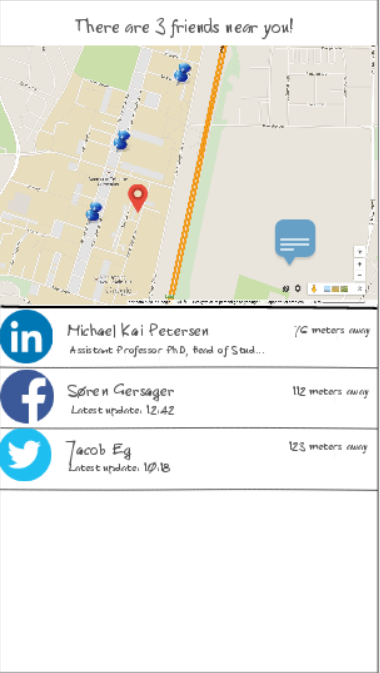
\includegraphics[width=0.6\textwidth]{figures/lo-fi-4}
\label{fig:lo-fi-fixed-panel-simple-marker}
\end{figure}

\begin{figure}
\centering
\caption{lo-fi prototype iteration 2}
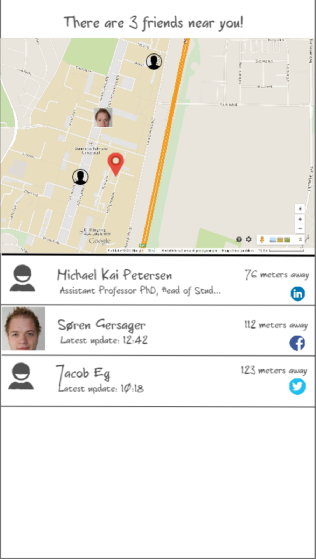
\includegraphics[width=0.6\textwidth]{figures/lo-fi-3}
\label{fig:lo-fi-fixed-panel}
\end{figure}

\begin{figure}
\centering
\caption{lo-fi prototype iteration 3, panel collapsed}
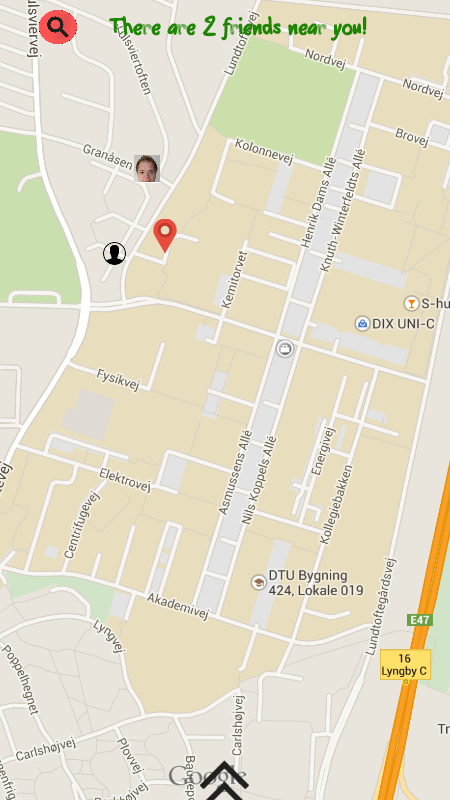
\includegraphics[width=0.6\textwidth]{figures/lo-fi-2}
\label{fig:lo-fi-panel-collapsed}
\end{figure}

\begin{figure}
\centering
\caption{lo-fi prototype iteration 3 w. navigation, panel expanded}
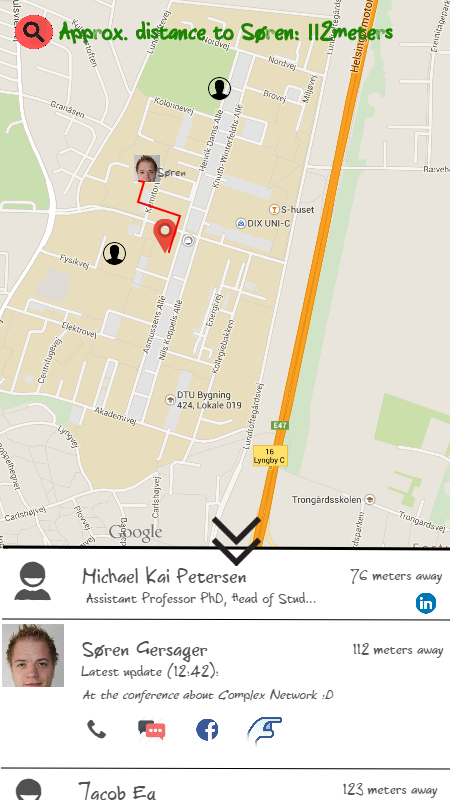
\includegraphics[width=0.6\textwidth]{figures/lo-fi-1}
\label{fig:lo-fi-w.navigation}
\end{figure}

\begin{figure}
\centering
\caption{Case before visualization, panel collapsed}
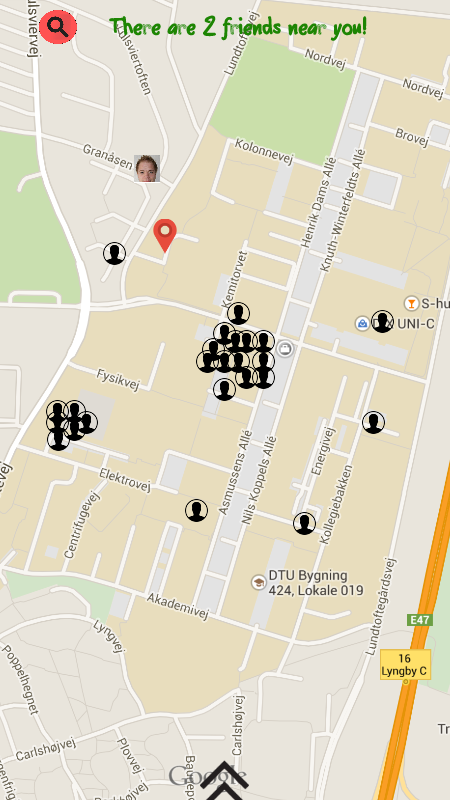
\includegraphics[width=0.6\textwidth]{figures/lo-fi-5}
\label{fig:before-visualization}
\end{figure}

\begin{figure}
\centering
\caption{final hi-fi prototype, panel expanded}
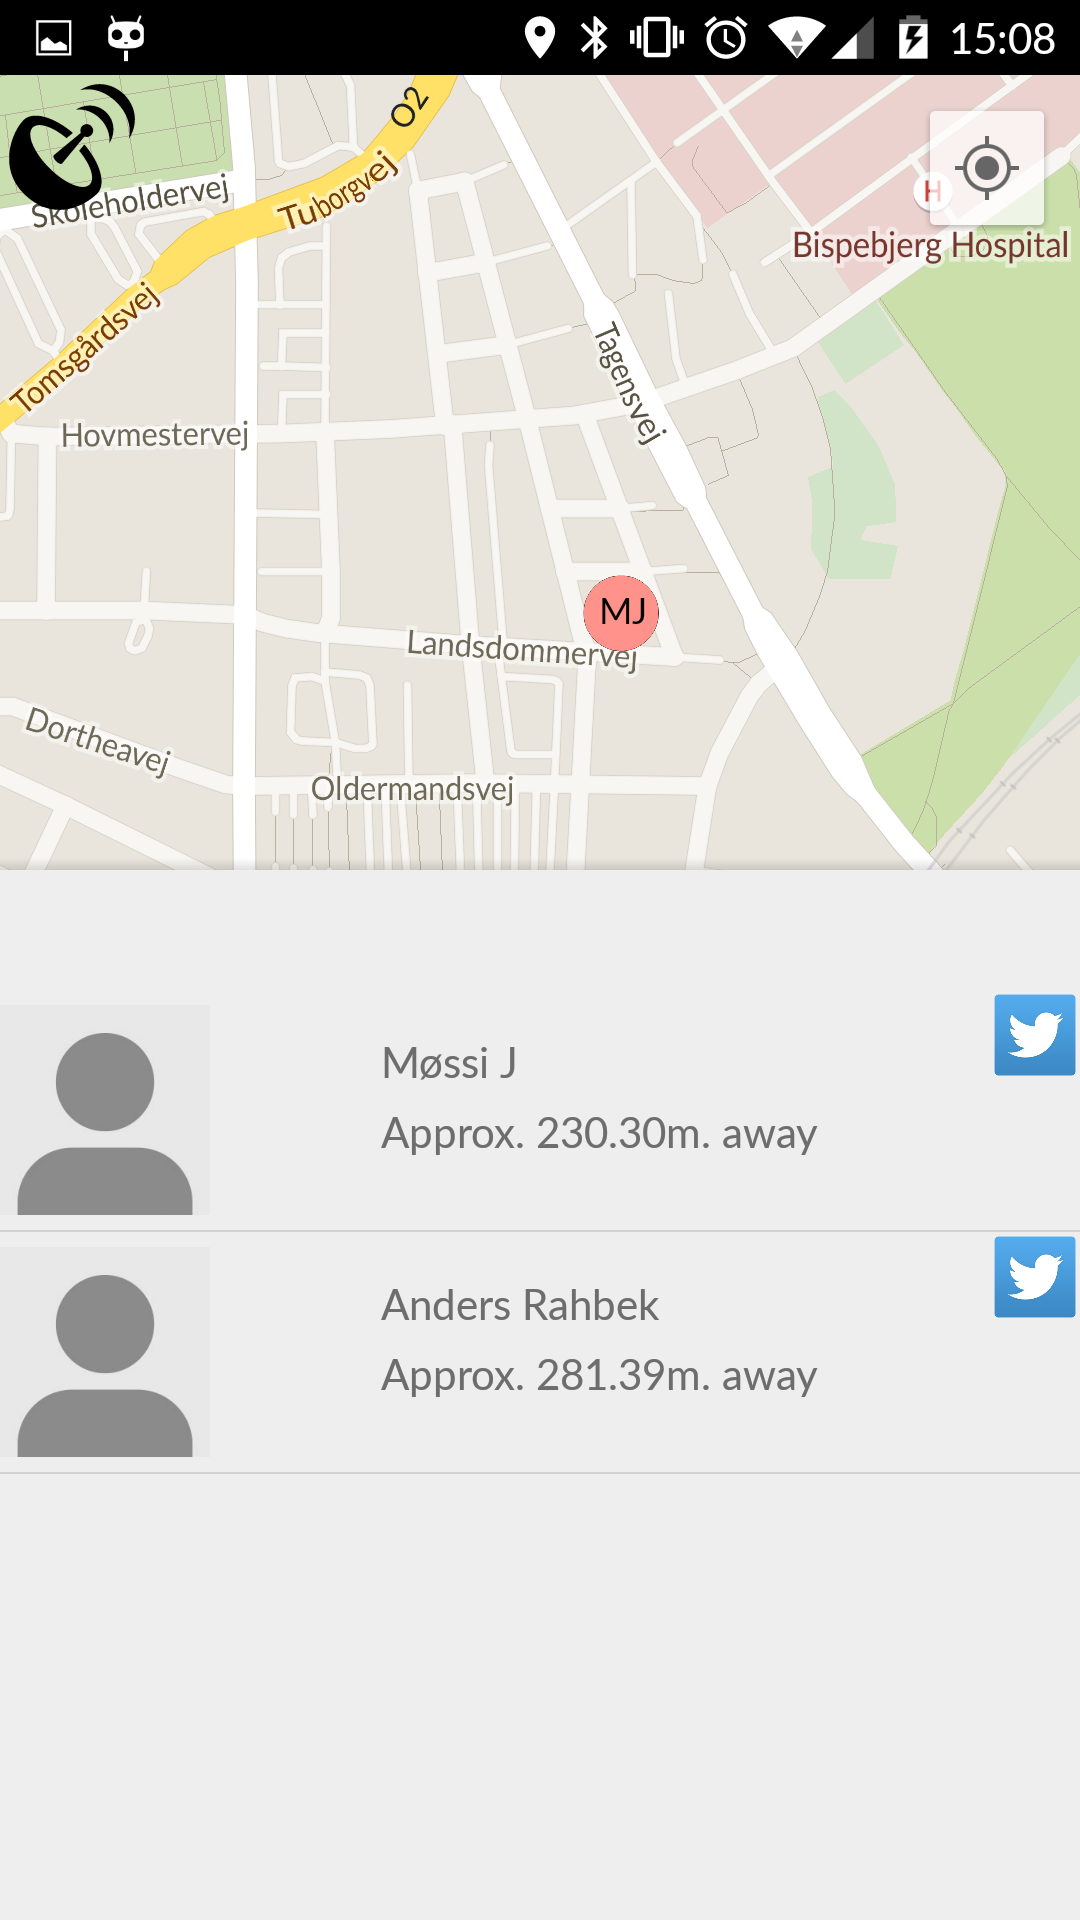
\includegraphics[width=0.6\textwidth]{figures/hi-fi-friendlist-expanded}
\label{fig:hi-fi app friendlist expanded}
\end{figure}

\begin{figure}
\centering
\caption{final hi-fi prototype, panel collapsed}
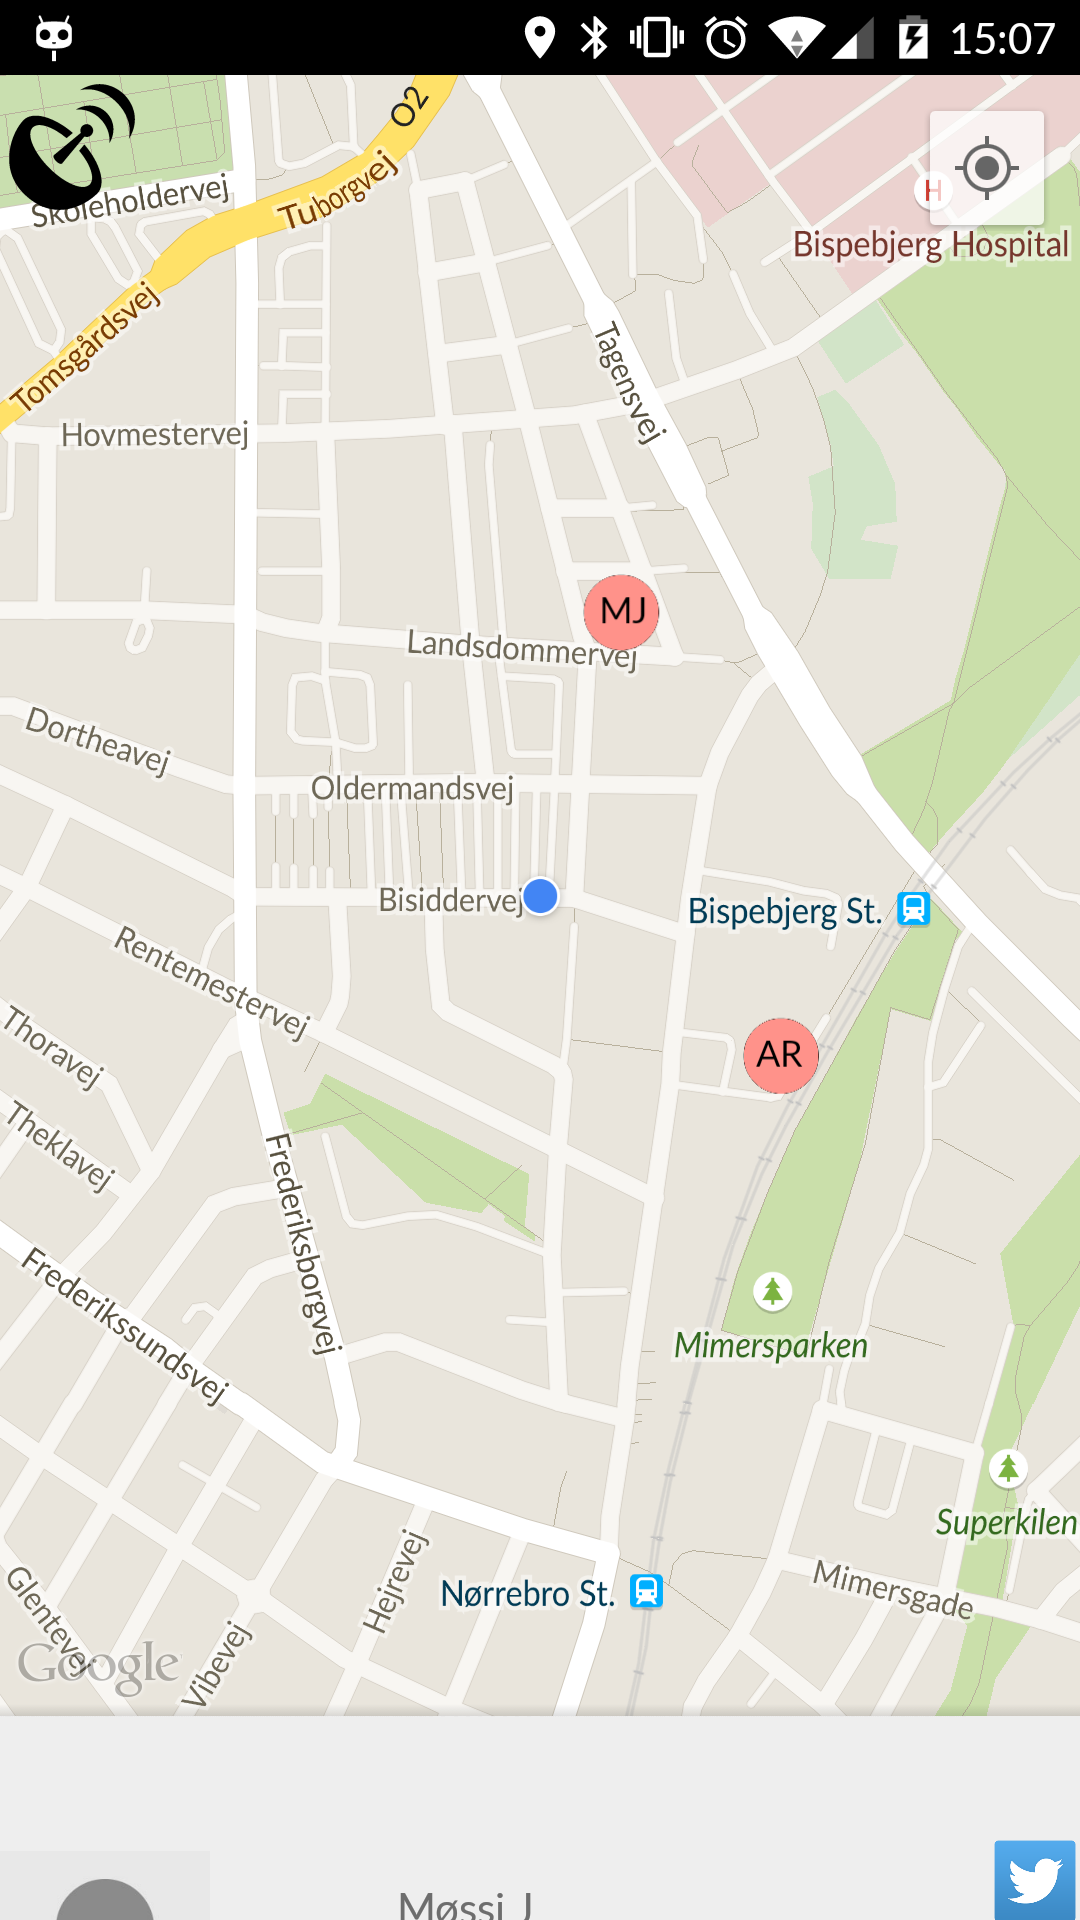
\includegraphics[width=0.6\textwidth]{figures/hi-fi-friendlist-collapsed}
\label{fig:hi-fi app friendlist collapsed}
\end{figure}

\begin{figure}
\centering
\caption{final hi-fi prototype, notification}
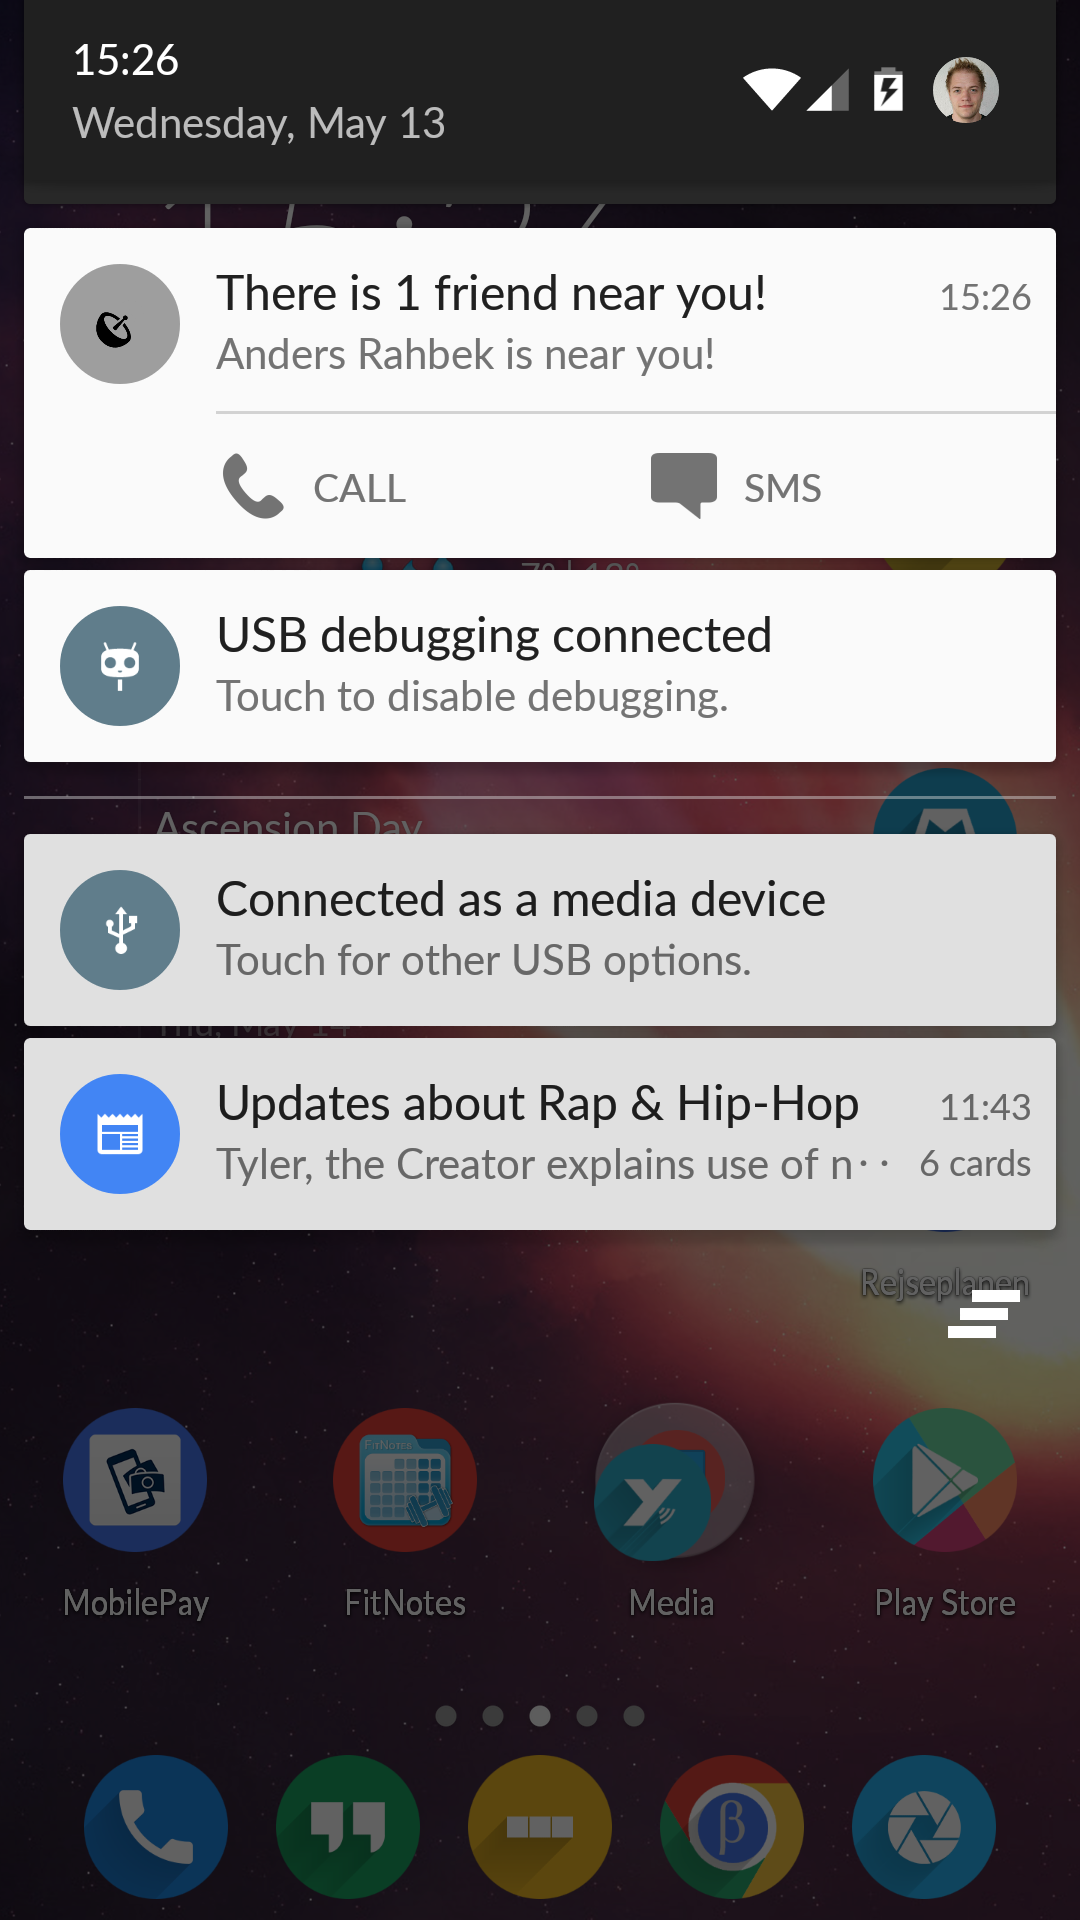
\includegraphics[width=0.6\textwidth]{figures/hi-fi-notification-app}
\label{fig:hi-fi app notification}
\end{figure}

\begin{figure}
\centering
\caption{final hi-fi prototype, watch notification collapsed}
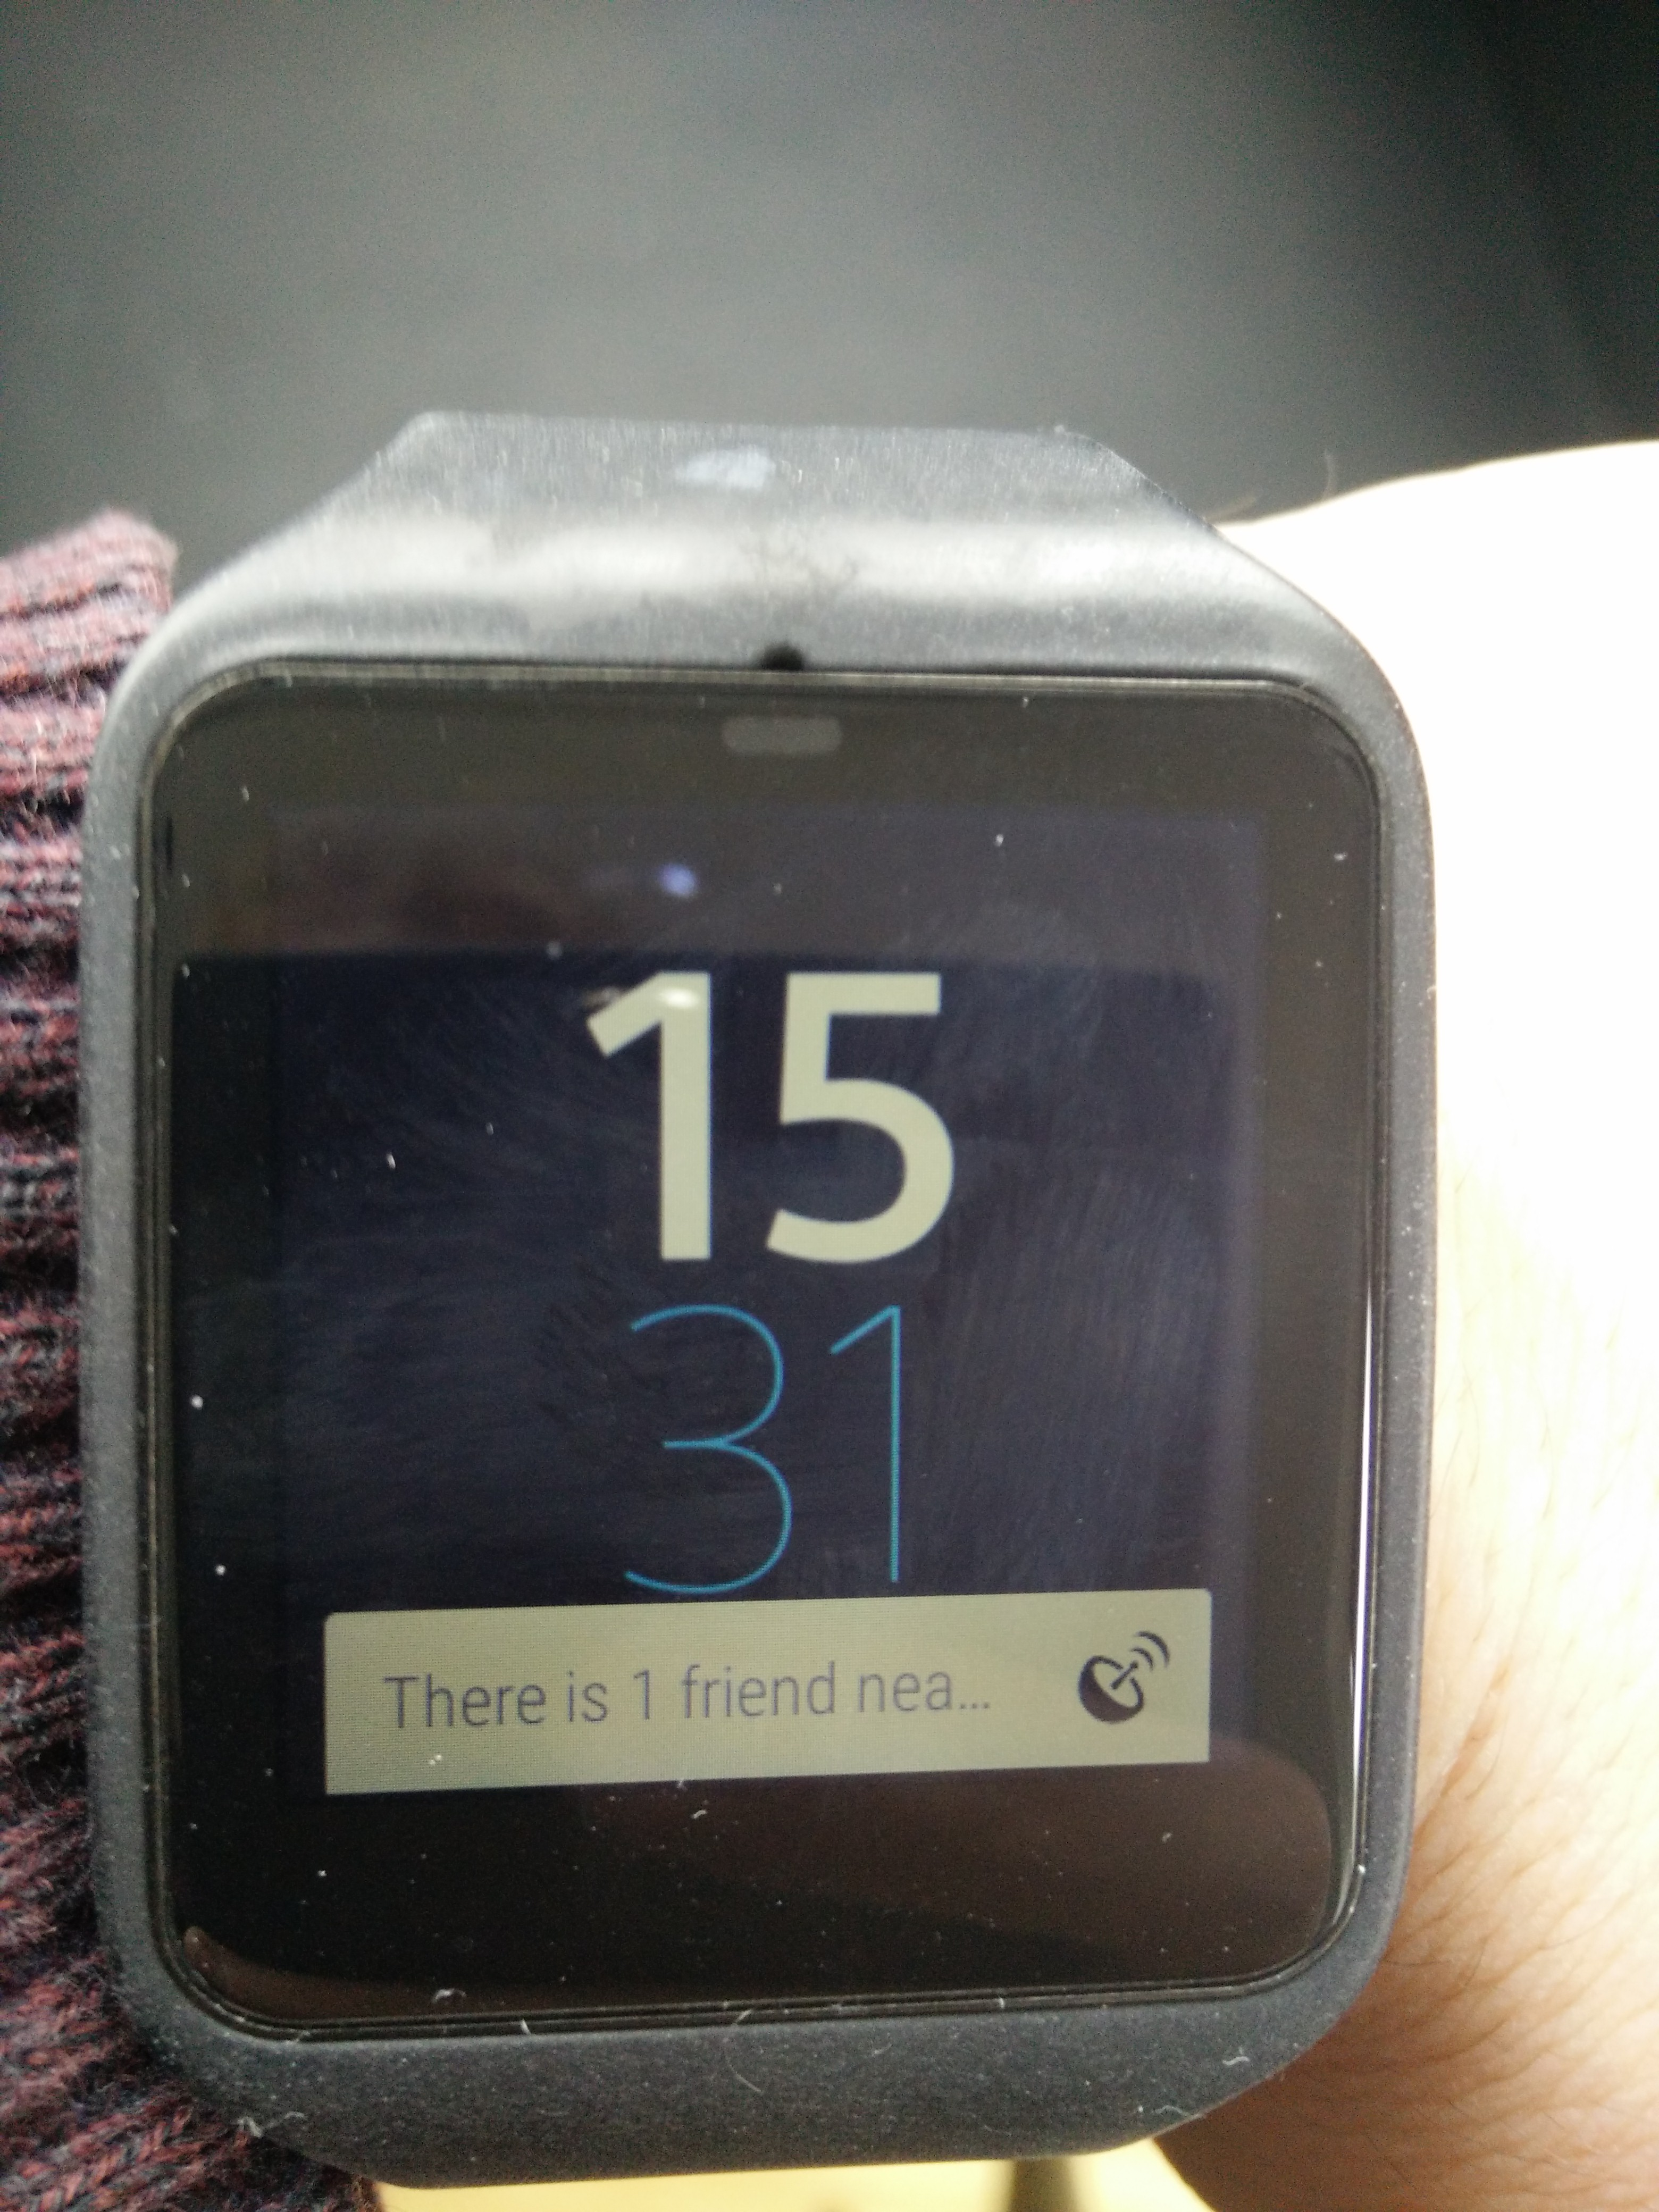
\includegraphics[width=0.6\textwidth]{figures/hi-fi-watch-collapsed}
\label{fig:hi-fi watch notification collapsed}
\end{figure}

\begin{figure}
\centering
\caption{final hi-fi prototype, watch notification expanded}
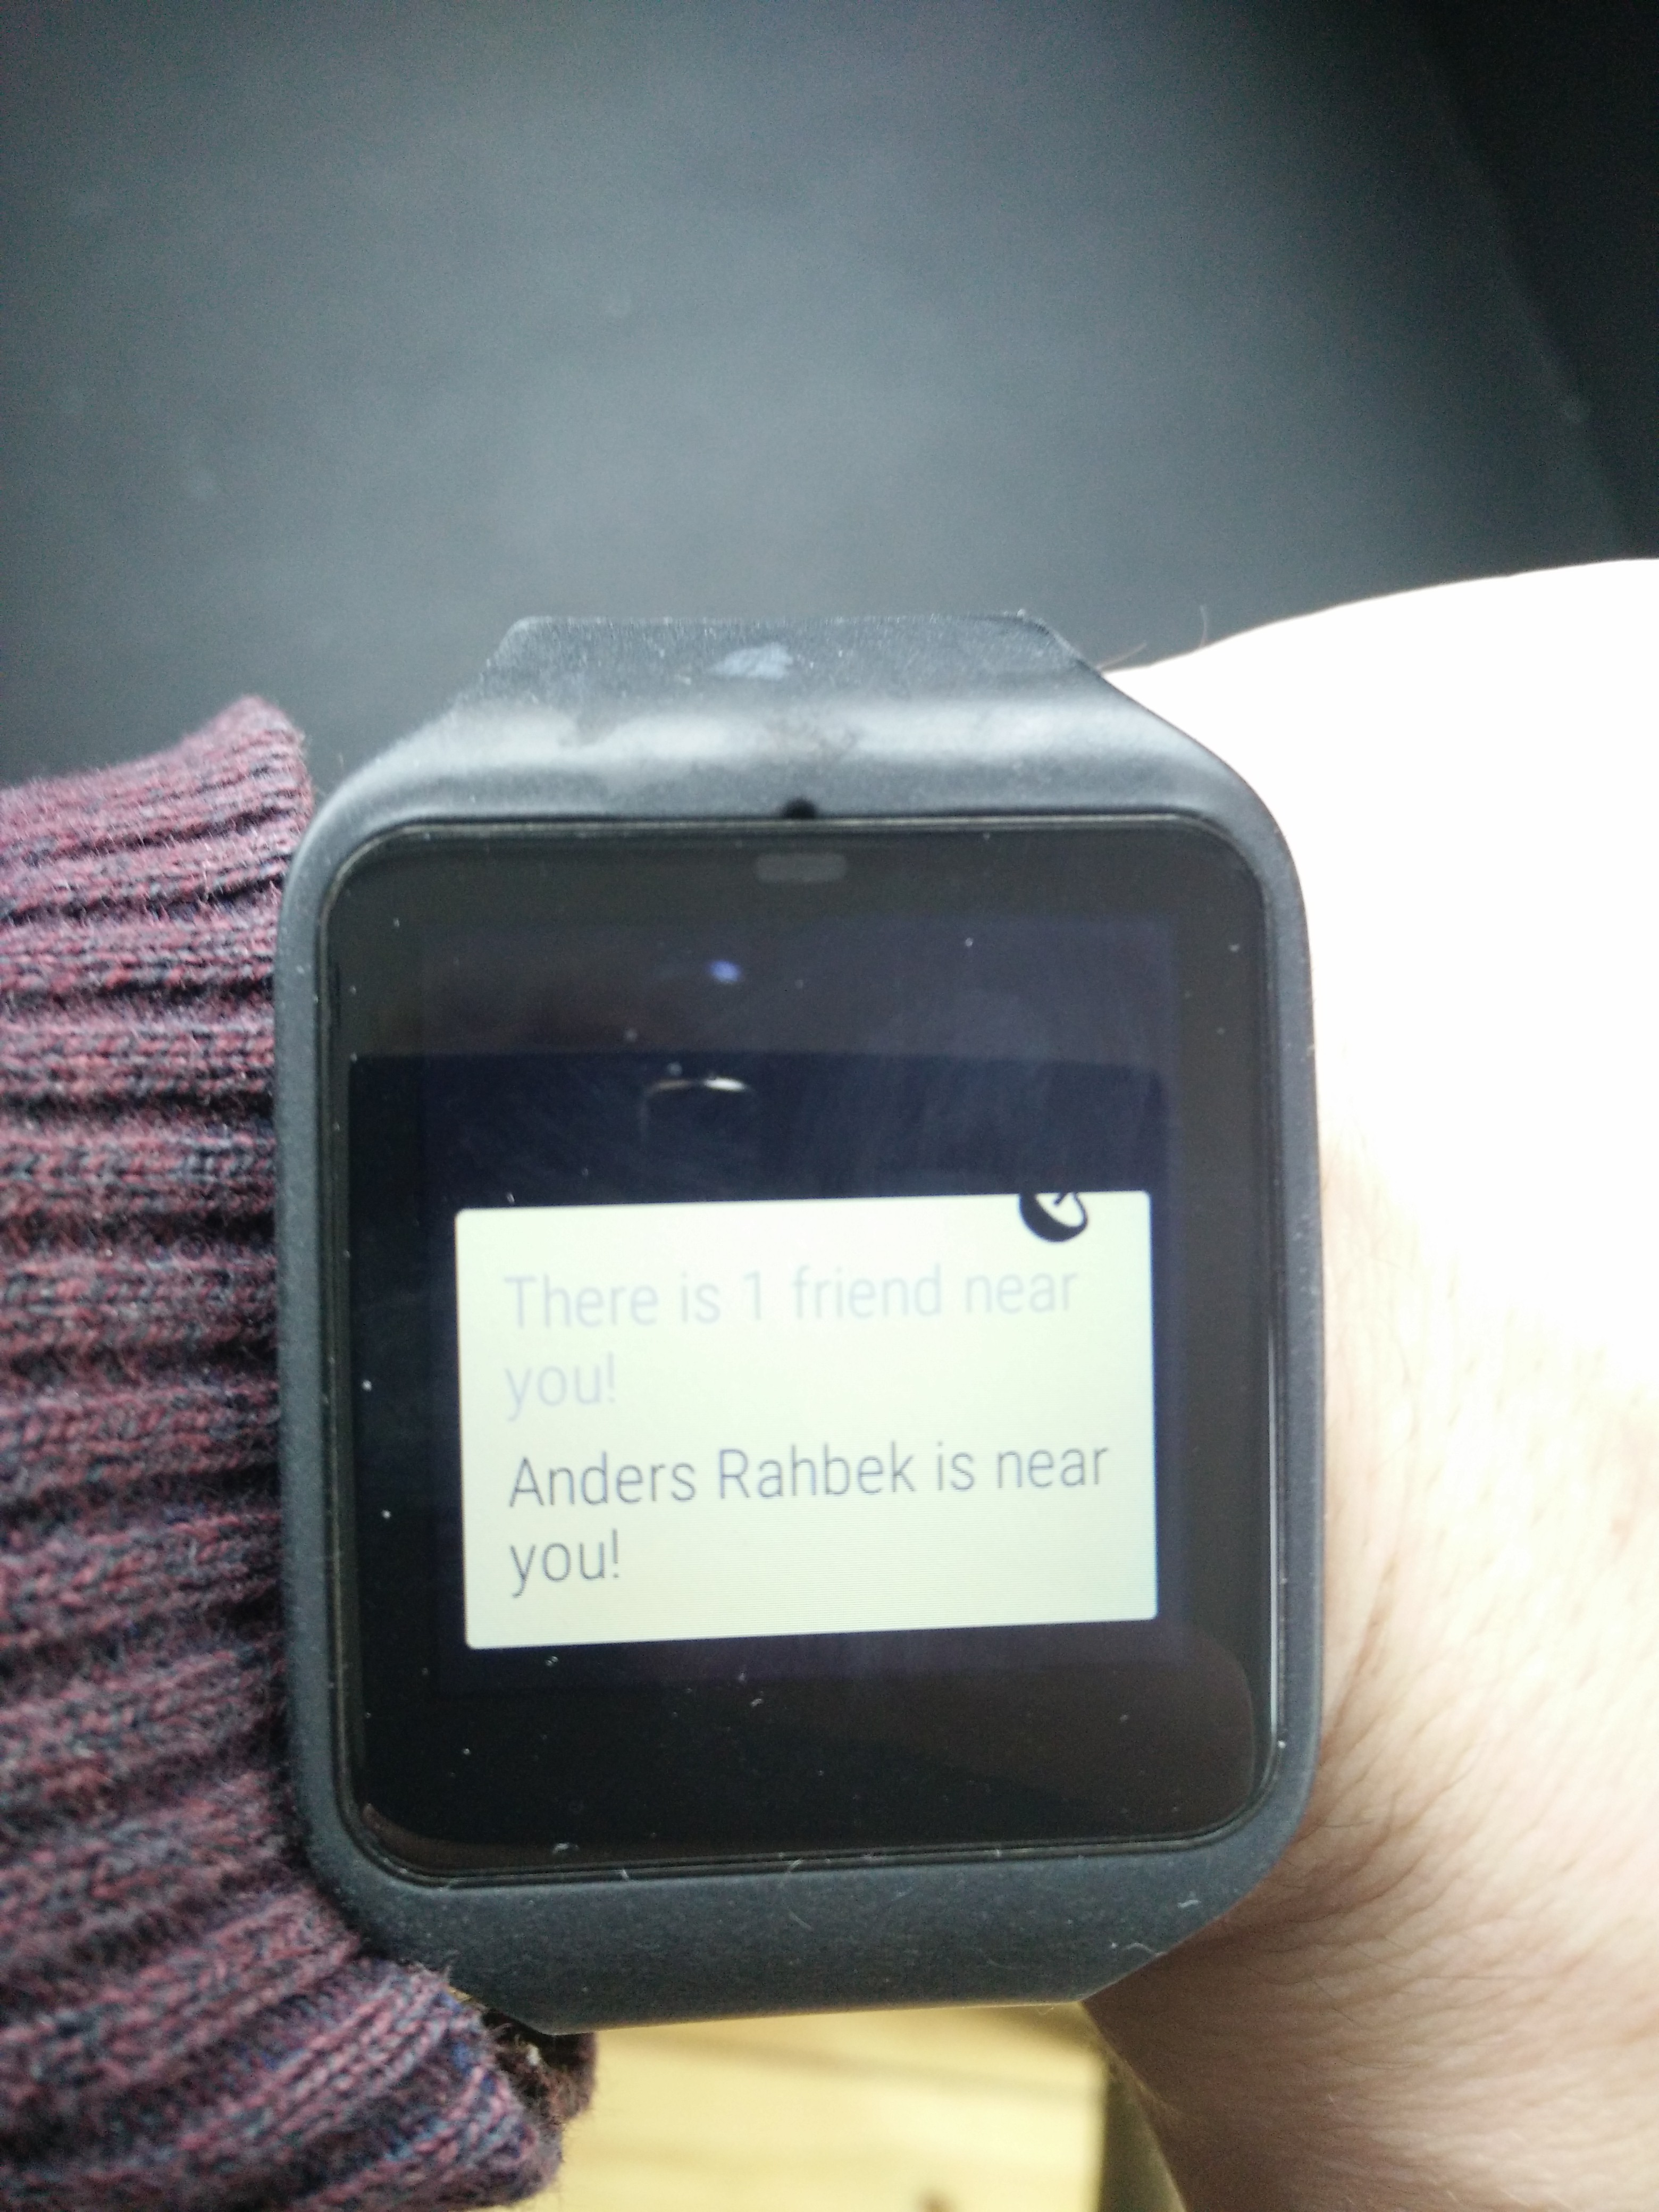
\includegraphics[width=0.6\textwidth]{figures/hi-fi-watch-expanded}
\label{fig:hi-fi watch notification expanded}
\end{figure}

\begin{figure}
\centering
\caption{final hi-fi prototype, watch call option}
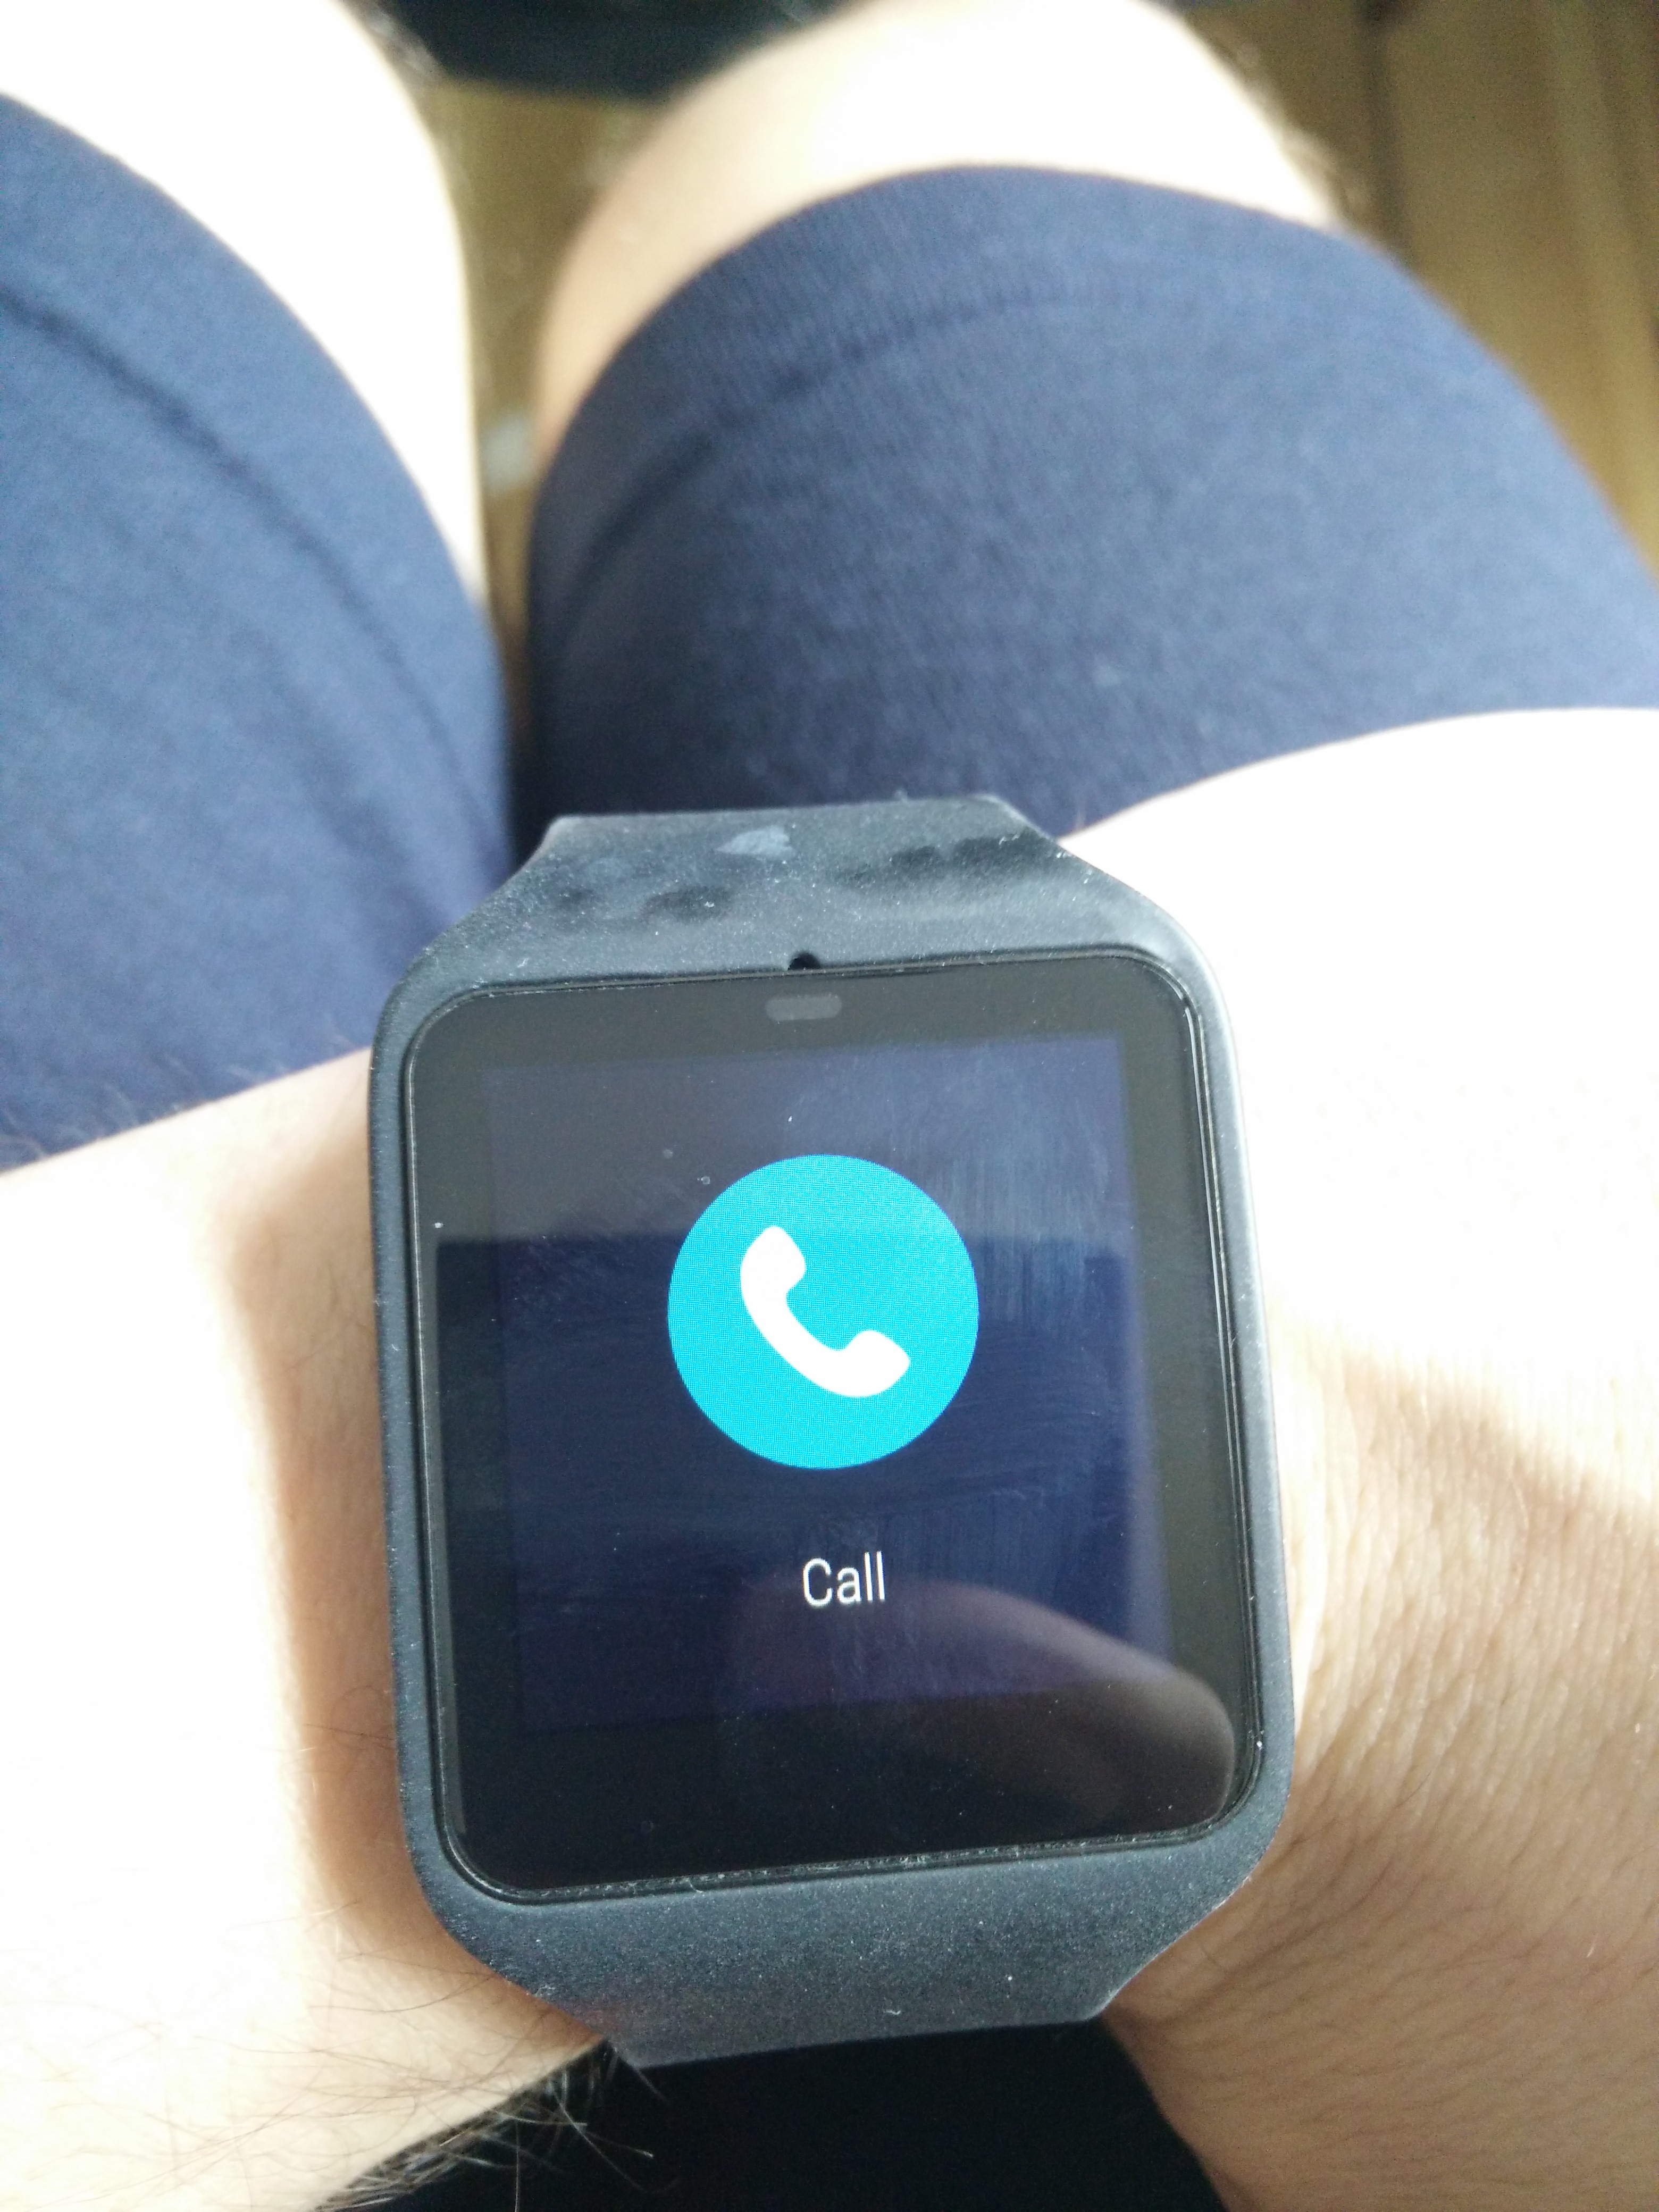
\includegraphics[width=0.6\textwidth]{figures/hi-fi-watch-call}
\label{fig:hi-fi watch call}
\end{figure}

\begin{figure}
\centering
\caption{final hi-fi prototype, watch sms}
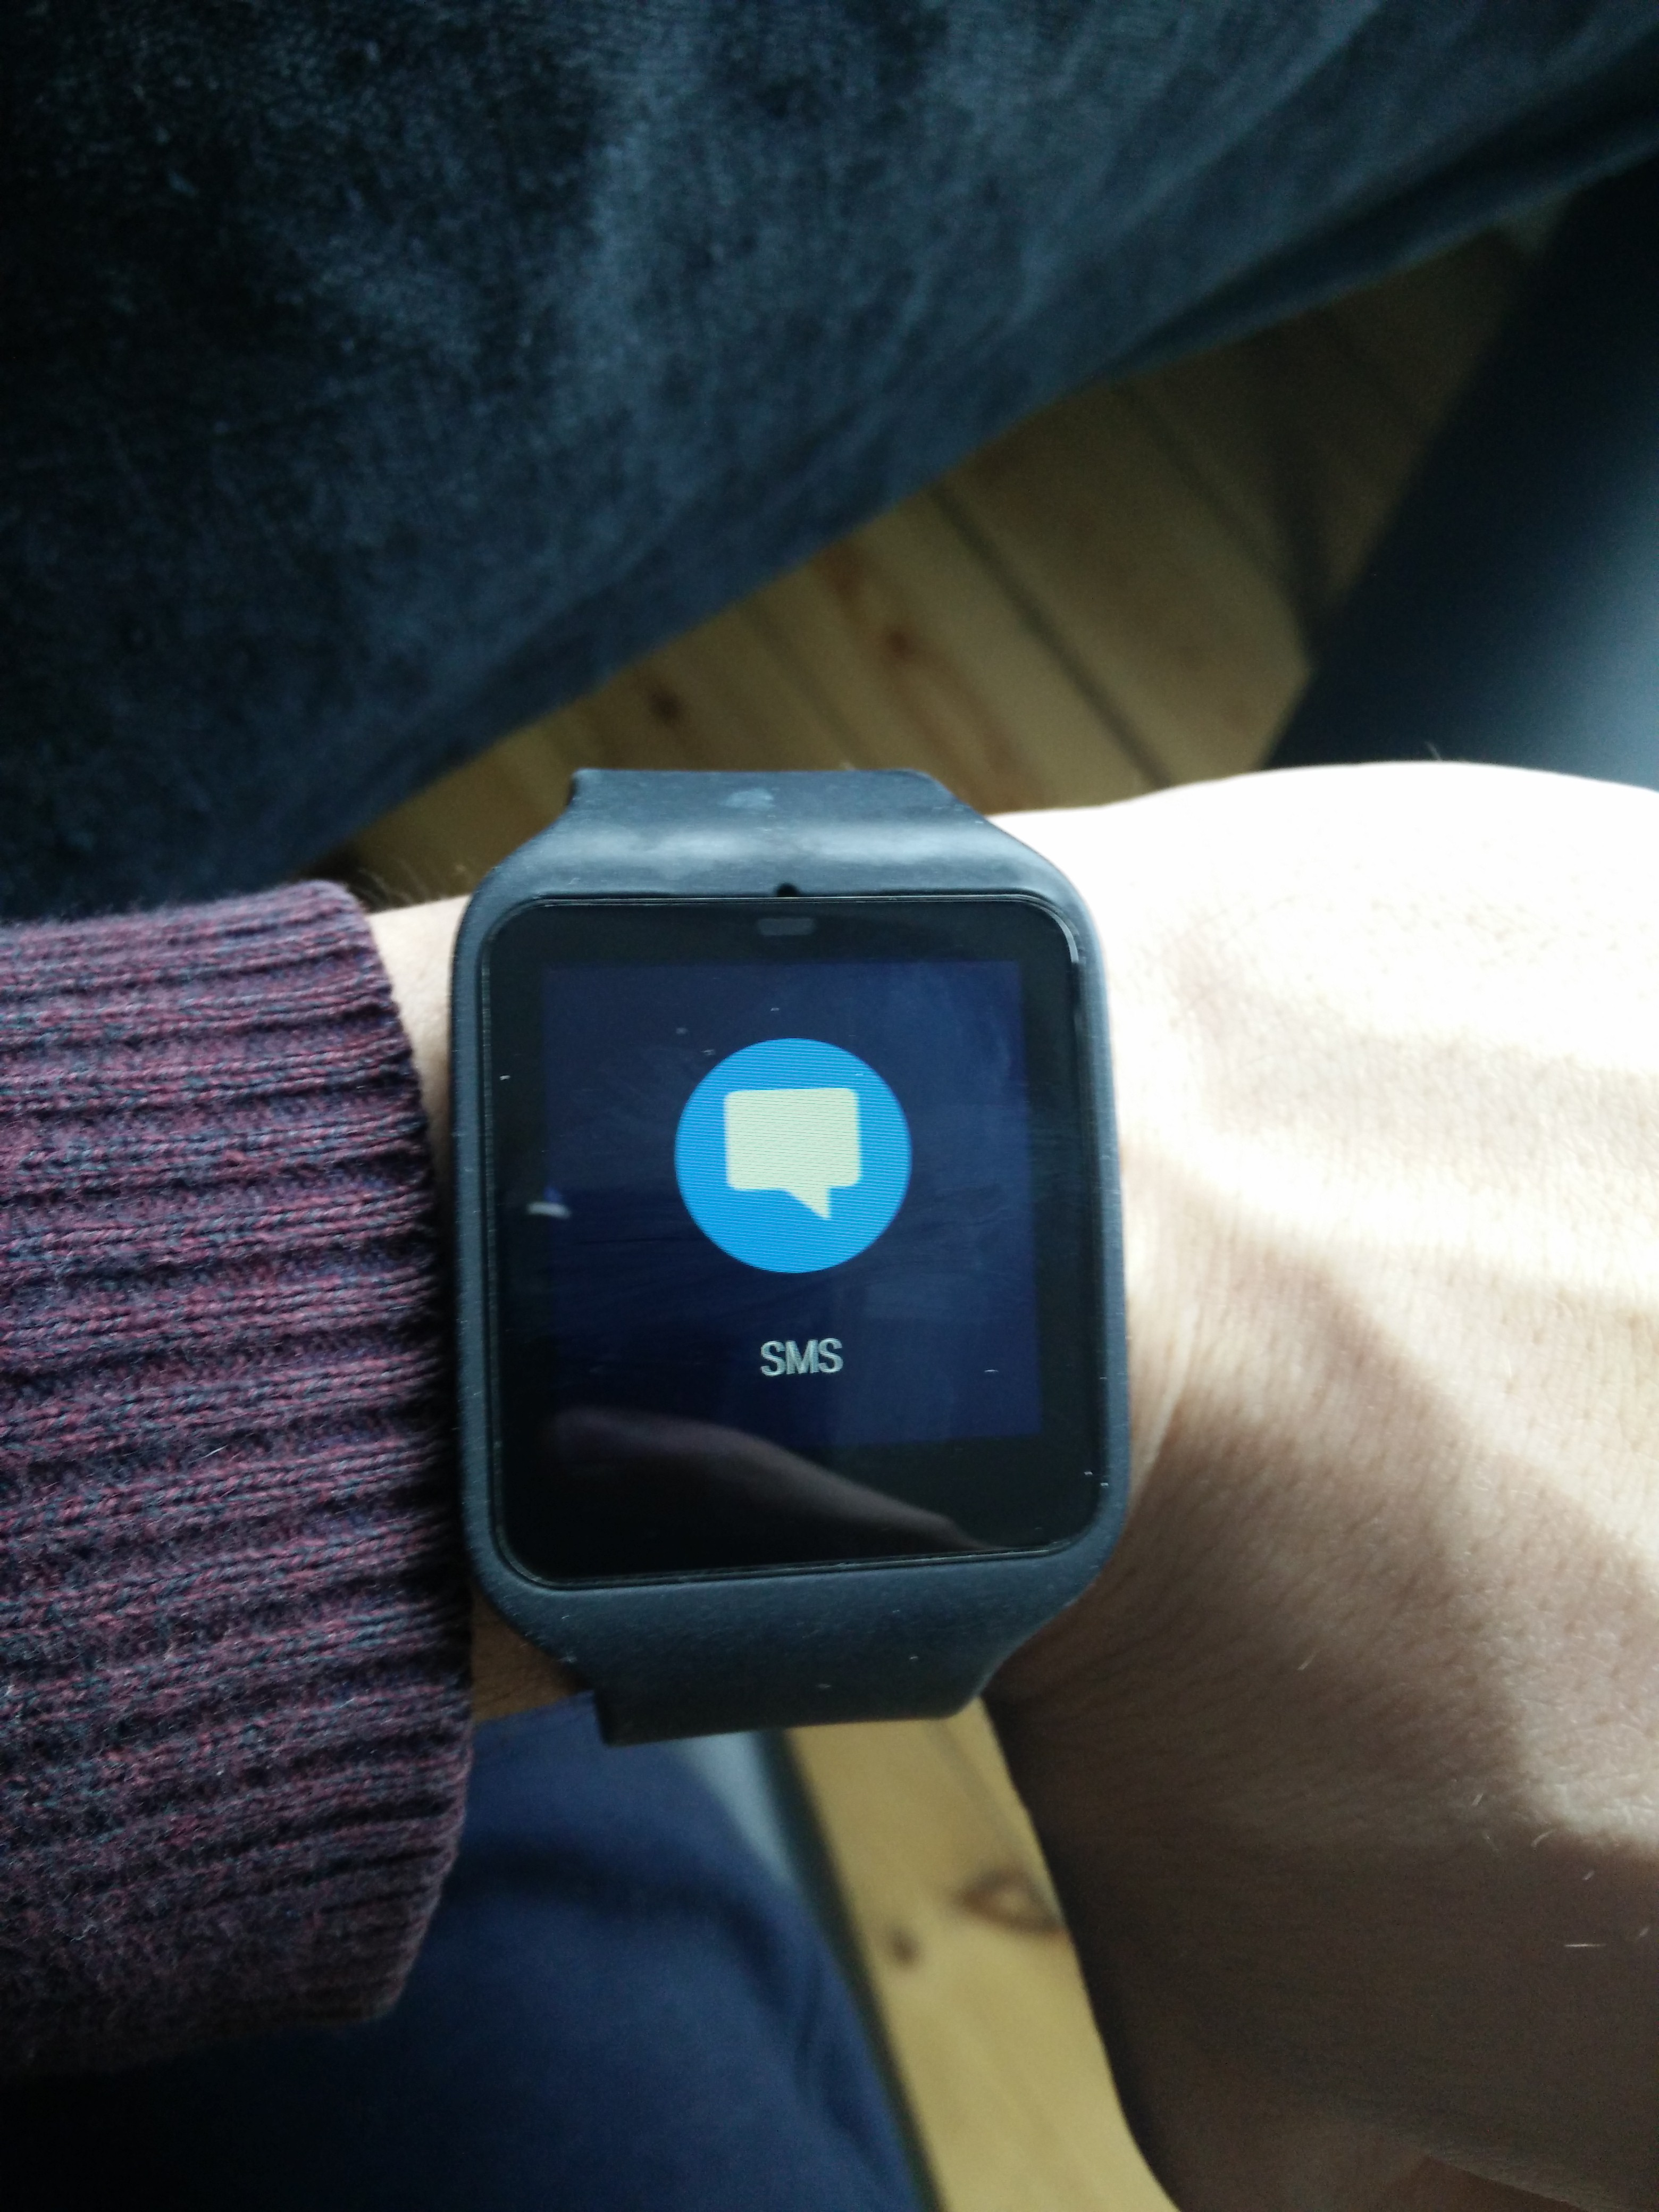
\includegraphics[width=0.6\textwidth]{figures/hi-fi-watch-sms}
\label{fig:hi-fi watch sms}
\end{figure}


\begin{figure}
\centering
\caption{Case after visualization, panel collapsed}
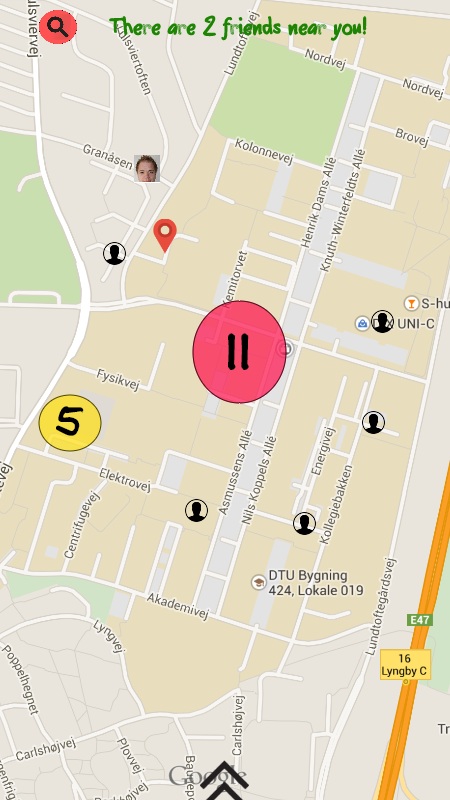
\includegraphics[width=0.6\textwidth]{figures/lo-fi-6}
\label{fig:after-visualization}
\end{figure}

\begin{figure}
\centering
\caption{Sequence diagram over onLocationChanged}
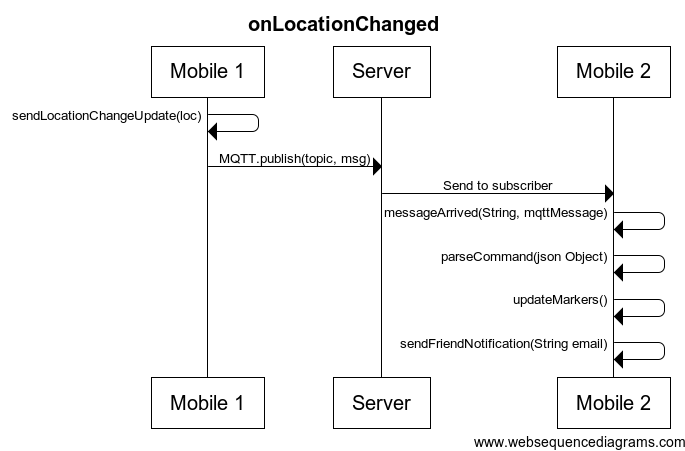
\includegraphics[scale=0.5]{figures/sq-1}
\label{fig:sq-onLocation}
\end{figure}

\begin{figure}
\centering
\caption{Sequence diagram over send Nudge}
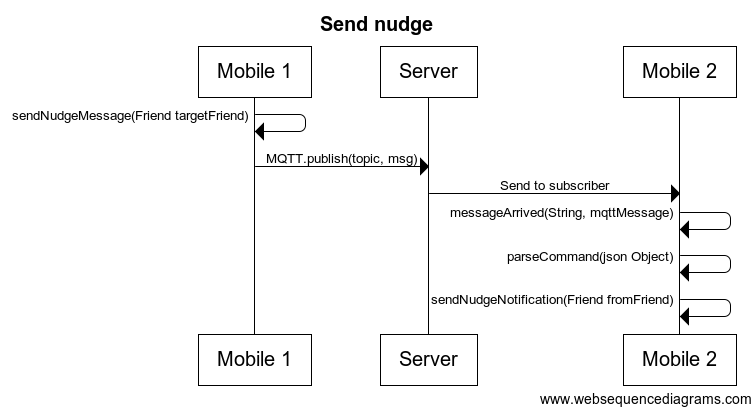
\includegraphics[scale=0.5]{figures/sq-2}
\label{fig:sq-nudge}
\end{figure}

\newgeometry{bottom=0.1cm}
\begin{landscape}
\begin{figure}
\caption{User story map for inception of initial lo-fi prototype}
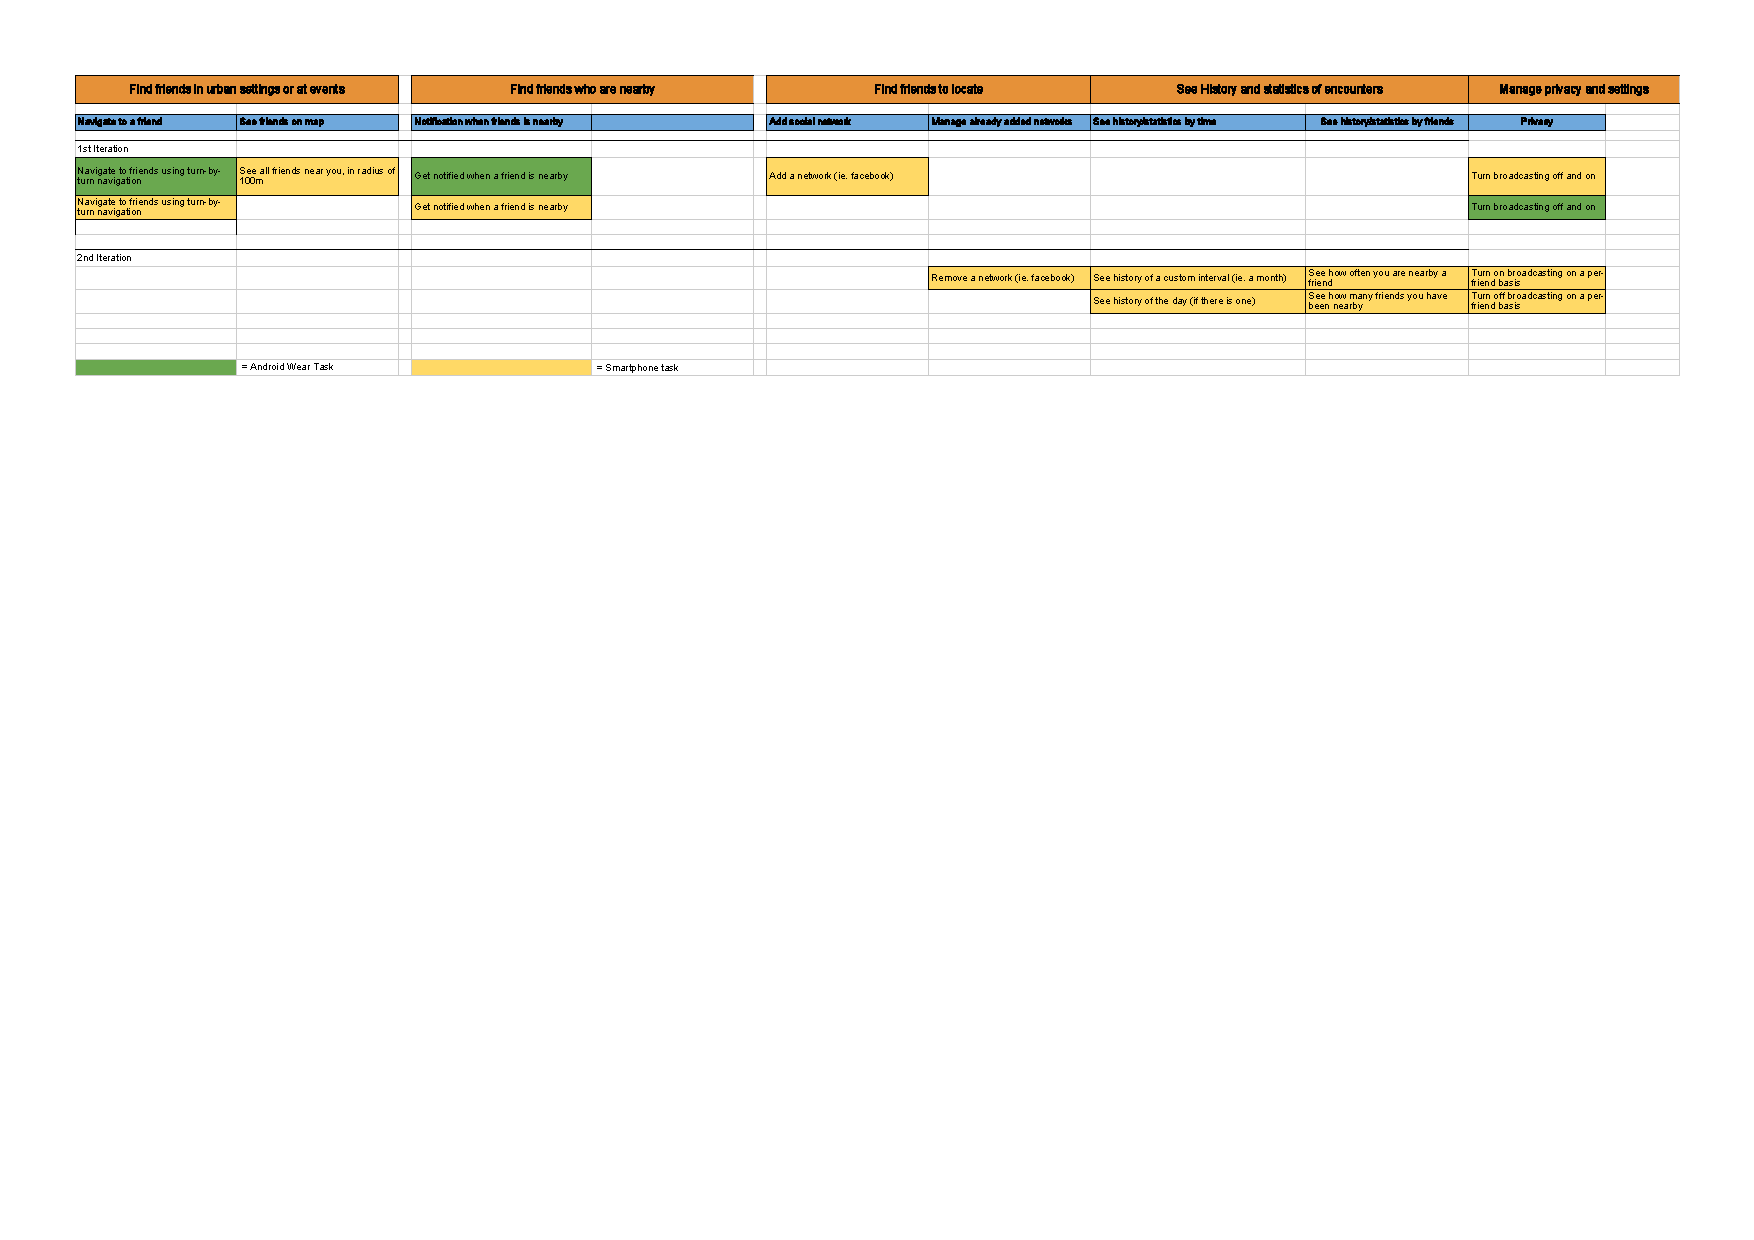
\includegraphics{figures/user_story_mapping}
\label{fig:user_story_mapping}
\end{figure}
\restoregeometry
\end{landscape}
\restoregeometry

\newgeometry{left=1.5cm, right=1.5cm}

\subsection*{Sourcecode} \label{source-code}
\lstset{numbers=left,
tabsize=1, numbersep=10pt,
  title=\lstname }
\lstinputlisting[language=Java]{FriendBump/mobile/src/main/java/com/example/syre/friendbump/MainActivity.java}
\newpage
\lstinputlisting[language=Java]{FriendBump/mobile/src/main/java/com/example/syre/friendbump/FriendListAdapter.java}
\newpage
\lstinputlisting[language=Java]{FriendBump/mobile/src/main/java/com/example/syre/friendbump/Friend.java}
\newpage
\lstinputlisting[language=Java]{FriendBump/mobile/src/main/java/com/example/syre/friendbump/GetFriends.java}
\restoregeometry
\end{document}
